\documentclass{beamer}
\usetheme{Boadilla}
\usepackage{tikz}
\usepackage{graphicx}
\usepackage{amsmath}
\usetikzlibrary{shapes.geometric,arrows, positioning, fit}




\title{Weekly Presentation}
\subtitle{Week 41}
\author{}
\institute{Luleå University of Technology}
\date{\today}



\begin{document}
\begin{frame}
    \titlepage
\end{frame}

\begin{frame}
    \frametitle{Overview}
    \tableofcontents
\end{frame}

%%%%%%%%%%%% Add new frames below this line %%%%%%%%%
\section{Status update}
%\begin{frame}
    \subsection{Time plan}
    \frametitle{Overall timetable}
    \begin{table}
        \begin{tabular}{| l | c | c | c | c }
            
            Sep & Oct & Nov & Dec \\
            \hline \hline
            Concept generation & Evaluation & Evaluation &  \\ 
            \hline
            Theory & Prototyping & Evaluation & Finishing up \\
            \hline
            Simulation & Evaluation & Evaluation & \\
            \hline
            Prototyping & Final Design & Evaluation &  \\
            \hline
 
        \end{tabular}
    \end{table}    
\end{frame}


\begin{frame}
    \frametitle{Time plan for September}
    \begin{table}
        \begin{tabular}{l | c | c | c | c }
        Subproject & Week 1 & Week 2 & Week 3 & Week 4 \\
        \hline \hline
            Arrowhead & Reading& Setup & API & Prototyping\\
            Movable base & Reading& Modeling & Simulation & Implementation\\
            Arm and grip  & Reading & Kinematics & Simulation& Prototyping\\
            Object detection & Reading & Testing & Prototyping & Evaluation\\
        \end{tabular}
    \end{table}
\end{frame}
\subsection{Milestone review}
\begin{frame}
    \frametitle{Finished}
    \begin{figure}
        \resizebox{7.0cm}{!}{
        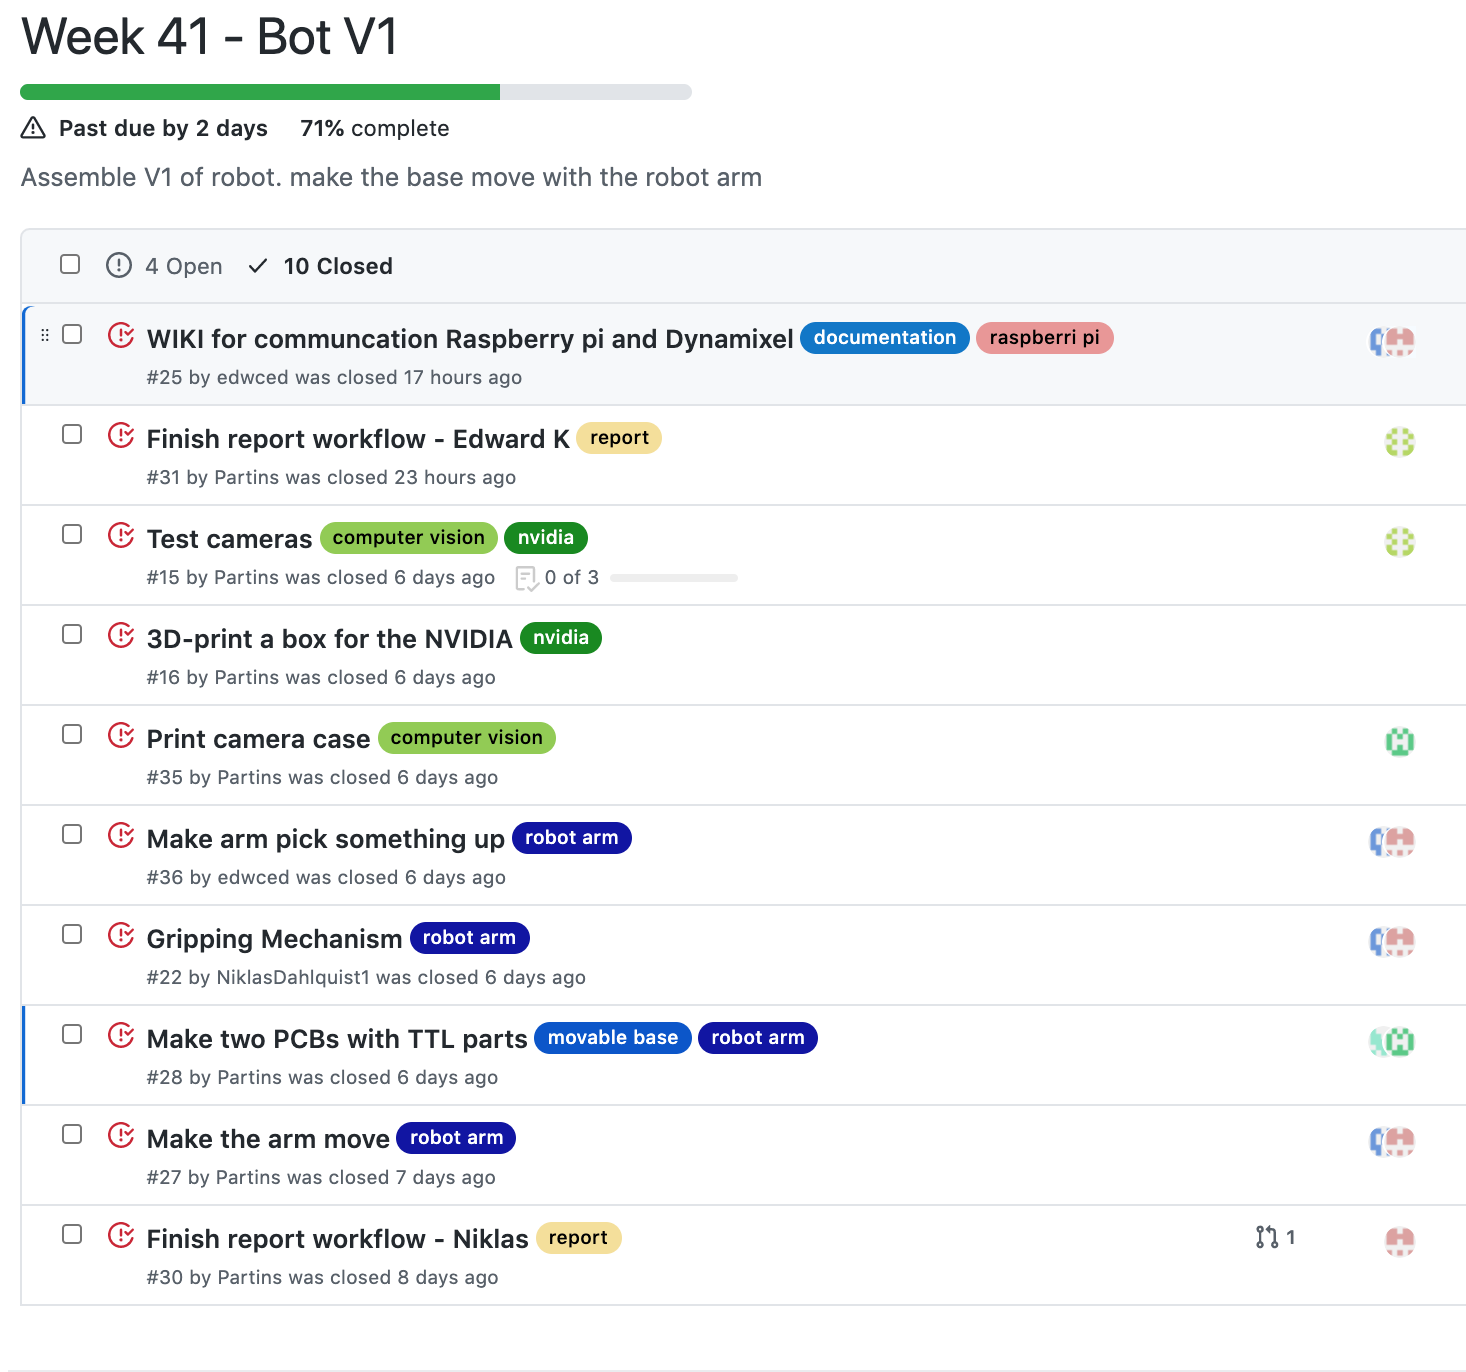
\includegraphics[width=\textwidth]{frames/img/milestone_week41_finished.png}
        }
    \end{figure}
\end{frame}

\begin{frame}
    \frametitle{Unfinished}
    \begin{figure}
        \resizebox{7.0cm}{!}{
        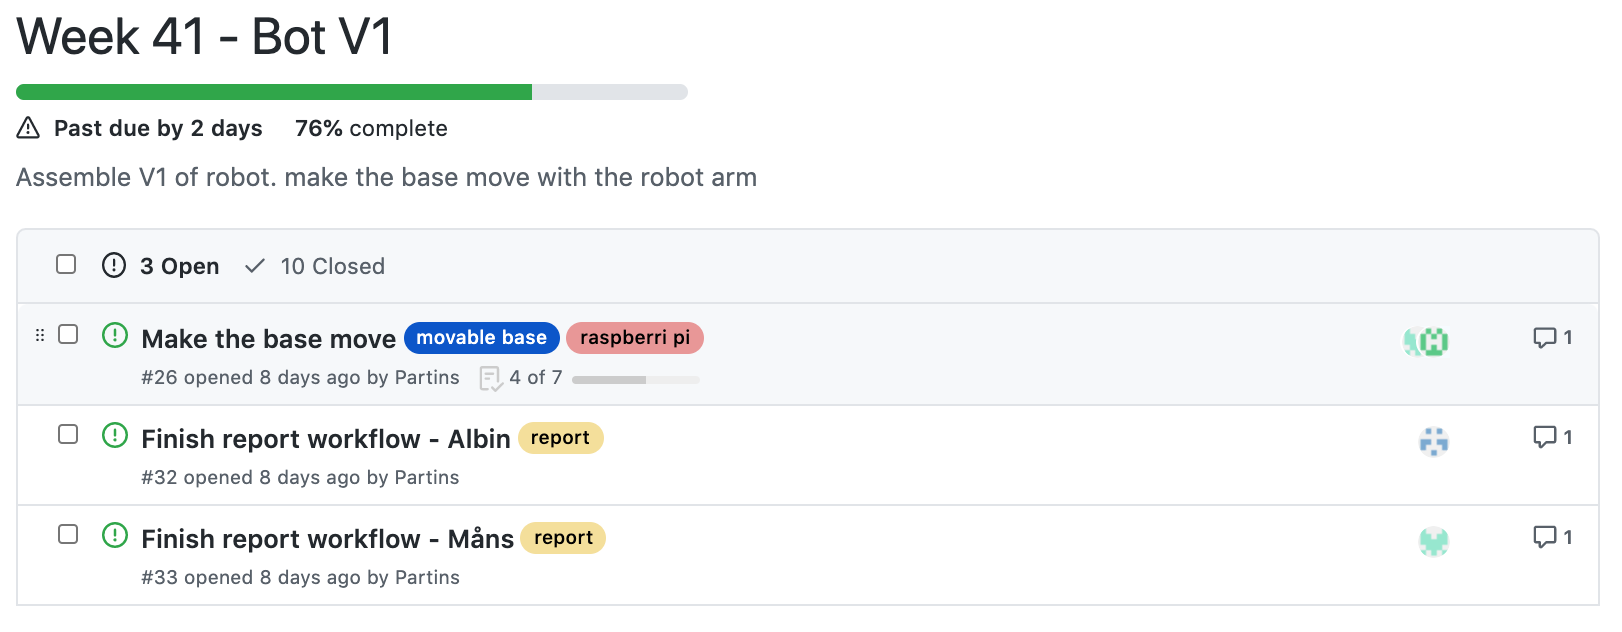
\includegraphics[width=\textwidth]{frames/img/milestone_week41_unfinished.png}
        }
    \end{figure}
\end{frame}

\begin{frame}
    \frametitle{Weekly plan}
    \begin{figure}
        \resizebox{7.0cm}{!}{
        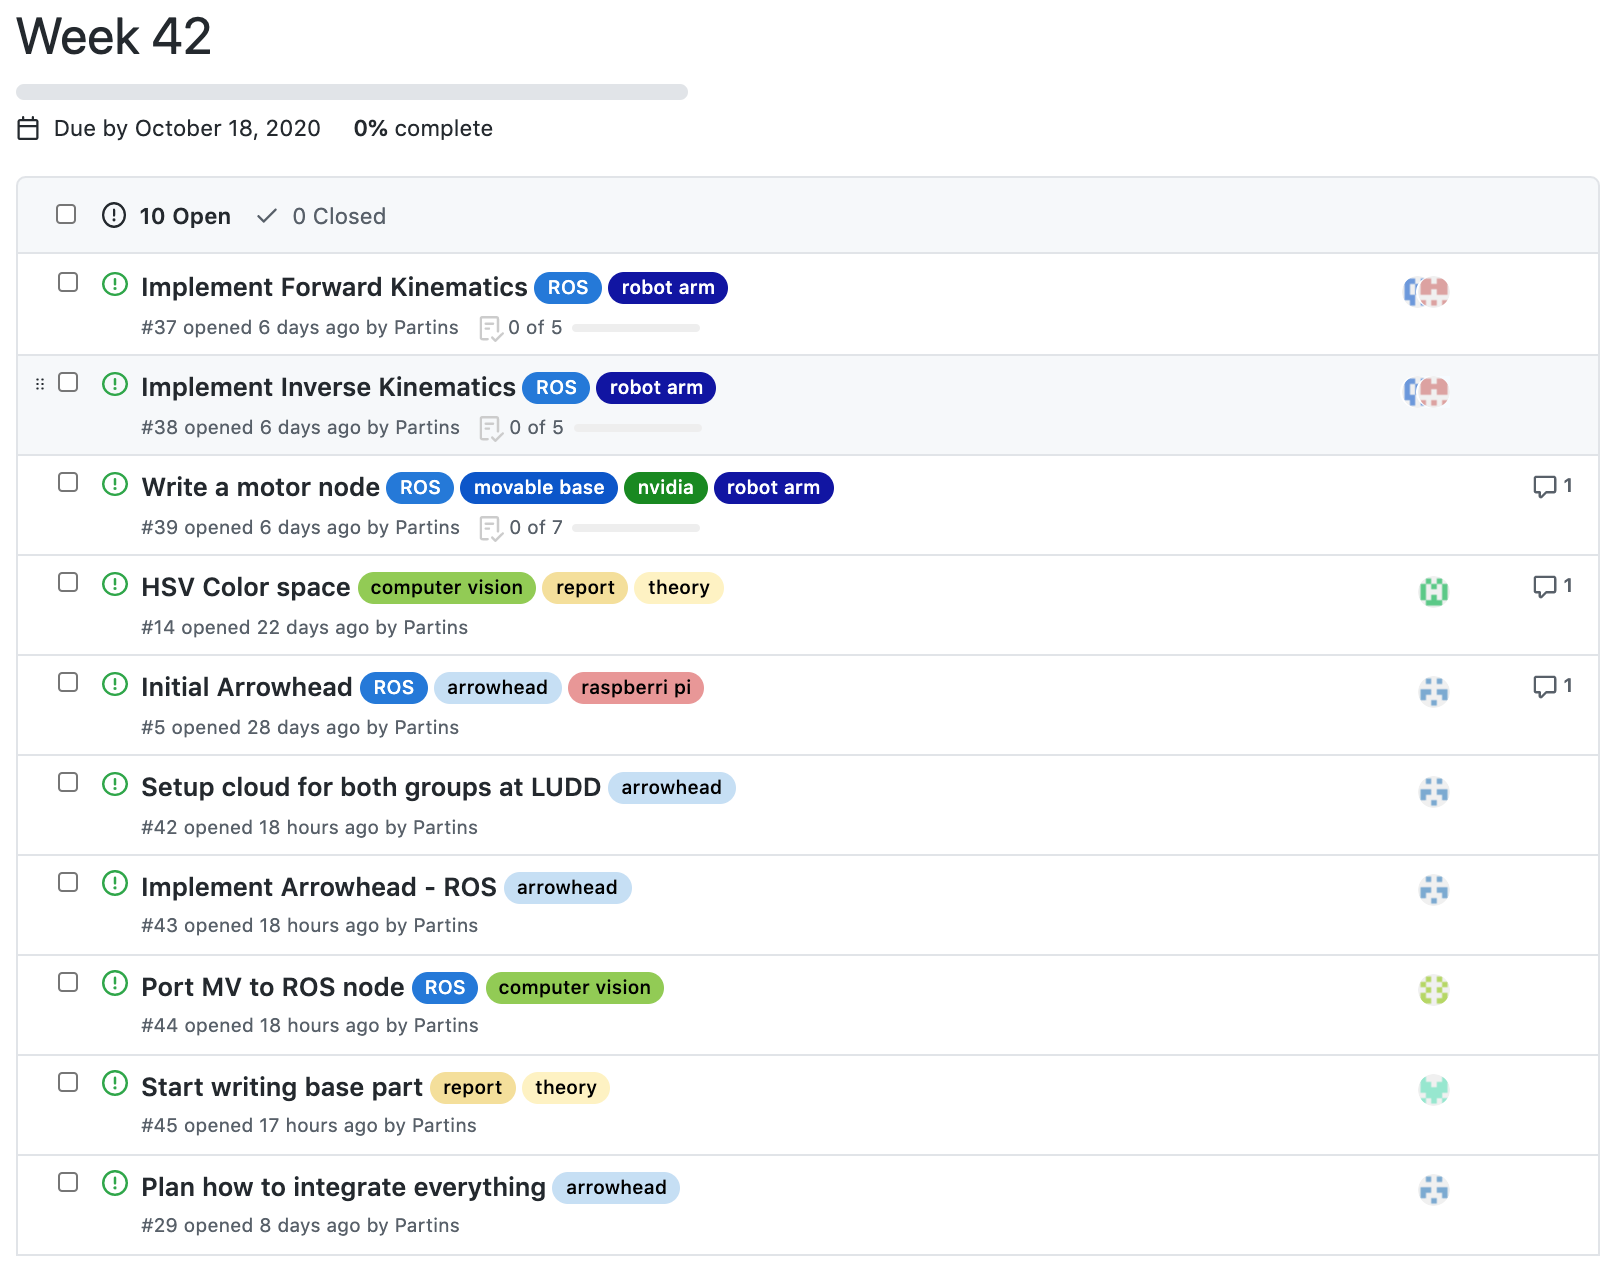
\includegraphics[width=\textwidth]{frames/img/milestone_week42.png}
        }
    \end{figure}
\end{frame}
\subsection{Challenges}
\begin{frame}
    \frametitle{Challenges}

    \begin{itemize}
        \item TTL communication on NVIDIA
        \begin{itemize}
            \item Ordered a USB-converter
        \end{itemize}
        \item Wheel mode gives no feedback
        \begin{itemize}
            \item Not needed for line following
            \item We know the distance of QR codes
        \end{itemize}
        \item Can't get HTTPS work with C++ (Arrowhead)
        \begin{itemize}
            \item More on that soon
        \end{itemize}
    \end{itemize}
\end{frame}

\section{Arrowhead}

\section{Computer Vision}


%%%%%%%%%%%% Add new frames above this line %%%%%%%%%


\begin{frame}
    \begin{center}
        \Huge Questions?
    \end{center}
\end{frame}





\end{document}